\documentclass[10pt,a4paper]{article}
\usepackage{amsmath}
\usepackage{amssymb}
\usepackage{graphicx}
\usepackage{color}
\usepackage{fancyhdr}
\usepackage{fancyvrb}
\usepackage[margin=3.5cm]{geometry}
\usepackage{framed}
\usepackage{enumerate}
\usepackage{textcomp}
\def\ket#1{\left|#1\right\rangle}
\def\bra#1{\left\langle#1\right|}
\def\braket#1{\left\langle#1\right\rangle}

\definecolor{linkcol}{rgb}{0.0, 0.0, 0.5}
\usepackage[colorlinks=true,urlcolor=linkcol,citecolor=black,linkcolor=linkcol]{hyperref}

\setcounter{section}{5}
\renewcommand\thesection{\arabic{section}}
\renewcommand\thesubsection{\thesection.\arabic{subsection}}

\fancyhf{}
\lhead{\tiny Y.~D.~Chong (2018)}
\rhead{\scriptsize MH2801: Complex Methods for the Sciences}
\lfoot{}
\rfoot{\thepage}
\pagestyle{fancy}

\makeatletter
\def\PY@reset{\let\PY@it=\relax \let\PY@bf=\relax%
    \let\PY@ul=\relax \let\PY@tc=\relax%
    \let\PY@bc=\relax \let\PY@ff=\relax}
\def\PY@tok#1{\csname PY@tok@#1\endcsname}
\def\PY@toks#1+{\ifx\relax#1\empty\else%
    \PY@tok{#1}\expandafter\PY@toks\fi}
\def\PY@do#1{\PY@bc{\PY@tc{\PY@ul
\def\PYZdl{\char`\$}
\def\PYZhy{\char`\-}
\def\PYZsq{\char`\'}
\def\PYZdq{\char`\"}
\def\PYZti{\char`\~}

\begin{document}
\setcounter{page}{42}
    
\section{Complex Derivatives}
\label{complex-derivatives}

We have studied functions that take real inputs and give complex
outputs (e.g., complex solutions to the damped harmonic oscillator,
which are complex functions of time). For such functions, the
derivative with respect to its real input is much like the derivative
of a real function of real inputs. It is equivalent to taking the
derivatives of the real and imaginary parts, separately:
\begin{equation}
\frac{d\psi}{dx} = \frac{d\mathrm{Re}(\psi)}{dx} + i \frac{d\mathrm{Im}(\psi)}{dx}.
\end{equation}
Now consider the more complicated case of a function of a \emph{complex}
variable:
\begin{equation}
f(z) \in \mathbb{C}, \;\;\mathrm{where}\;\; z \in \mathbb{C}.
\end{equation}
At one level, we could just treat this as a function of two independent
real inputs: $f(x,y)$, where $z = x + i y$. However, in doing so we
would be disregarding the mathematical structure of the complex
input---the fact that $z$ is not just a mere collection of two real
numbers, but a complex \emph{number} that can be subjected to algebraic
operations. This structure has important implications for the
differential calculus of complex functions.

\subsection{Complex continuity and differentiability}
\label{complex-continuity-and-differentiability}

The concept of a \textbf{continuous complex function} is as follows:

\begin{framed} \noindent
A complex function $f(z)$ is continuous at $z_0 \in \mathbb{C}$ if,
for any $\epsilon > 0$, we can find a $\delta > 0$ such that
\[\big|\, z - z_0 \,\big| < \delta \;\;\; \Rightarrow \;\;\; \big|\, f(z) - f(z_0) \,\big| < \epsilon.\]
\end{framed}

\noindent
Here, $\big|\cdots\big|$ denotes the magnitude of a complex
number. This definition basically says that as we vary $z$ smoothly,
there should be no abrupt jumps in the value of $f(z)$.

If a function is continuous at a point $z$, we can define its
\textbf{complex derivative} as

\begin{framed} \noindent
  \begin{equation}
    f'(z) = \frac{df}{dz}
    = \lim_{\delta z\rightarrow 0} \frac{f(z+\delta z) - f(z)}{\delta z}.
  \end{equation}
\end{framed}

\noindent
This is very similar to the definition of the derivative for a
function of a real variable. However, there's a complication which
doesn't appear in the real case: the infinitesimal $\delta z$ is a
complex number, not just a real number. The above definition does not
specify the argument of the complex number.  The choice of the
argument of $\delta z$ is equivalent to the direction in the complex
plane in which $\delta z$ points, as shown in the following figure:

\begin{figure}[h]
  \centering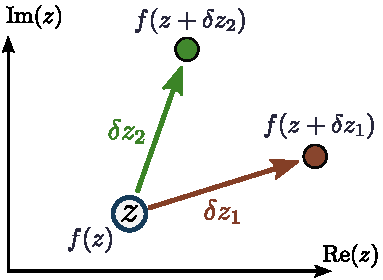
\includegraphics[width=0.4\textwidth]{complex_derivative}
\end{figure}

In principle, we might get different results from the above formula when
we plug in different infinitesimals $\delta z$, even in the limit
where $\delta z \rightarrow 0$ and even though $f(z)$ is continuous.

\begin{framed} \noindent
\textit{Example}---Consider the function $f(z) = z^*$. According to
the derivative formula,
\begin{equation*}
  \lim_{\delta z \rightarrow0} \frac{f(z+\delta z) - f(z)}{\delta z} = \lim_{\delta z \rightarrow0} \frac{z^*+\delta z^* - z^*}{\delta z} = \lim_{\delta z \rightarrow0} \frac{\delta z^*}{\delta z}.
\end{equation*}
But if we plug in a real $\delta z$, we get a different result than if
we plug in an imaginary $\delta z$:
\begin{align*}
  \delta z \in \mathbb{R} \;\; &\Rightarrow \frac{\delta z^*}{\delta z} = 1.\\
  \delta z \in i \cdot \mathbb{R} &\Rightarrow \frac{\delta z^*}{\delta z}
  = -1.
\end{align*}
\end{framed}

To cope with this complication, we regard the complex derivative as
well-defined \emph{only if} the above definition gives the same answer
regardless of the argument of $\delta z$. If a function satisfies this
property at $z$, we say that the function is
\textbf{complex-differentiable} at $z$.

As shown in the above example, $f(z) = z^*$ is not
complex-differentiable for any $z \in \mathbb{C}$. On the other hand,
the following example shows that the function $f(z) = z$ is
complex-differentiable for all $z \in \mathbb{C}$:

\begin{framed} \noindent
  \textit{Example}---We can prove that the function $f(z) = z$ is
  complex differentiable for any $z \in \mathbb{C}$, as
  follows:
\begin{equation}
  \lim_{\delta z \rightarrow0} \frac{f(z+\delta z) -
    f(z)}{\delta z} = \lim_{\delta z \rightarrow0} \frac{z+\delta z -
    z}{\delta z} = \lim_{\delta z \rightarrow0} \frac{\delta z}{\delta
    z} = 1.
\end{equation}
The reason the result doesn't depend on the argument of $\delta z$ is
that the derivative formula simplifies to the fraction $\delta z /
\delta z$. The value of this fraction is 1 for any $|\delta z| > 0$.
\end{framed}

\subsection{Analytic functions}\label{analytic-functions}

If a function $f(z)$ is complex-differentiable for all points $z$ in
some domain $D\subset \mathbb{C}$, then $f(z)$ is said to be
\textbf{analytic} in $D$.

The concepts of analyticity and complex-differentiability are closely
related. It's mainly a matter of terminology: we speak of a function
being complex-differentiable \emph{at a given point}, whereas we speak
of a function being analytic \emph{in a given domain}.

\begin{framed} \noindent
\textit{Example}---As shown in the preceding section, $f(z) = z$ is
complex-differentiable for any point $z \in \mathbb{C}$. Thence,
$f(z) = z$ is analytic in $\mathbb{C}$.
\end{framed}

A function's domain of analyticity is usually described spatially, in
terms of parts of the complex plane. For example, a function might be
analytic ``everywhere in the complex plane'', which means the entire
domain $\mathbb{C}$. Or a function might be analytic ``in the upper
half of the complex plane'', meaning for all $z$ such that
$\mathrm{Im}(z) > 0$.

\subsubsection{Common analytic functions}
\label{common-analytic-functions}

There is an important class of functions which are analytic over the
entire complex plane, or most of the complex plane. These are
functions generated from algebraic formulas which do not contain
$z^*$, and involve $z$ in some ``simple'' combination of operations
like addition, multiplication, and integer powers.

For example, we have seen that the function $f(z) = z$ is analytic in
$\mathbb{C}$. Likewise, $f(z) = \alpha z + \beta$, where $\alpha,
\beta$ are complex constants, is analytic everywhere in
$\mathbb{C}$. This can be proven in a similar fashion:
\begin{align}
  f'(z) &= \lim_{\delta z\rightarrow 0} \frac{[\alpha\,(z+\delta z) + \beta] - [\alpha z + \beta]}{\delta z} \\&= \lim_{\delta z\rightarrow 0} \frac{\alpha \delta z}{\delta z} \\&= \alpha.
\end{align}
We can also show that $f(z) = z^n$, with $n \in \mathbb{N}$, is
analytic everywhere in $\mathbb{C}$:
\begin{align}
  f'(z) &= \lim_{\delta z\rightarrow 0} \frac{(z+\delta z)^n - z^n}{\delta z} \\&=
  \lim_{\delta z\rightarrow 0} \frac{(z^n + n z^{n-1} \delta z + \cdots) - z^n}{\delta z} \\&= n z^{n-1}.
\end{align}
Note that these derivatives have exactly the same algebraic formulas as
the corresponding real derivatives. This is no coincidence: to derive
the complex derivatives, we take the same series of algebra steps used
for deriving the real derivatives.

From the discussion so far, it is evident that complex polynomials are
analytic everywhere in $\mathbb{C}$. Likewise, functions that are
defined in terms of power series, including the complex exponential
and complex sines and cosines, are analytic everywhere in
$\mathbb{C}$. Functions involving reciprocals (negative integer
powers), such as $f(z) = z^{-1}$ or $f(z) = z^{-2}$, are analytic
everywhere \emph{except} at points where $f(z)$ becomes singular
(i.e., the denominator goes to zero). (We will prove this Section
\ref{cauchy-riemann-equations}.) More generally, whenever a function
involves $z$ in some combination of integer polynomials, reciprocals,
or functions with power series expansions---and does not involve $z^*$
in an irreducible way---then the function is analytic everywhere
except at the singular points. Moreover, the formula for the complex
derivative is the same as the corresponding formula for real
derivatives.

\begin{framed} \noindent
  \textit{Example}---The function\[f(z) = \frac{1}{\cos(z)}\]is
  analytic everywhere in $\mathbb{C}$, except for values of $z$ such
  that $\cos(z) = 0$.  With a bit of work (try it!), one can show that
  these $z$ occur at isolated points along the real line, at $z =
  (m+1/2)\pi$ where $m \in \mathbb{Z}$, and nowhere else in the
  complex plane. The complex derivative is
\begin{equation*}
  f'(z) = \frac{\sin(z)}{[\cos(z)]^2}.
\end{equation*}
  The easiest way to prove these statements is to use the Cauchy
  Riemann equations, which are discussed in Section
  \ref{cauchy-riemann-equations}.
\end{framed}

One proviso should be kept in mind. For non-integer powers, $z^a$
where $a\notin \mathbb{Z}$, the situation is more complicated because
the operation is multi-valued. We'll postpone the discussion of these
special operations until the discussion on branch points and branch
cuts in the next chapter.

\subsubsection{Numerical example of an analytic function}
\label{numerical-example-of-an-analytic-function}

In the following Python example, we look at the complex derivative of
the function
\begin{equation}
f(z) = \sin(z),
\end{equation}
which is analytic everywhere in $\mathbb{C}$. The derivative can be
estimated numerically as
\begin{equation}
\frac{\delta f}{\delta z} = \frac{\sin(z + \delta z) - \sin(z)}{\delta z}
\end{equation}
for $\delta z$ with very small magnitude. Note that these are complex
numbers, since the sine and cosine functions give complex outputs when
the input $z$ is complex.

We observe that the numerical results are insensitive to the choice of
$\delta z$ (including real and imaginary values), so long as
$|\delta z|$ is small. In the limit where
$|\delta z| \rightarrow 0$, the value should become independent of
$\mathrm{arg}(z)$, and approach the limiting value of the complex
derivative:
\begin{equation}
\frac{df}{dz} = \lim_{|\delta z| \rightarrow 0} \frac{\delta f}{\delta z} = \cos(z).
\end{equation}

\subsection{The Cauchy-Riemann equations}
\label{cauchy-riemann-equations}

The \textbf{Cauchy-Riemann equations} are a pair of real partial
differential equations that provide an alternative way to understand
complex derivatives. Their importance comes from the following
theorem:

\begin{framed}\noindent
Let $f$ be a complex function that can be written as the sum of real
and imaginary parts, \[f(z = x + iy) \;=\; u(x,y) + i v(x,y),\] where
$u(x,y)$ and $v(x,y)$ are real functions of two real inputs. Then
$f$ is complex-differentiable at a given $z$ if and only if the
two equations
\begin{align}
  \frac{\partial u}{\partial x} &= \frac{\partial v}{\partial y} \label{cr1}\\
  \frac{\partial u}{\partial y} &= -\frac{\partial v}{\partial x} \label{cr2}
\end{align}
are well-defined and true.
\end{framed}

\noindent
The two partial differential equations \eqref{cr1} and \eqref{cr2} are
the Cauchy-Riemann equations. ``Well-defined'', in the context of this
theorem, means that the functions $u(x,y)$ and $v(x,y)$ must have
valid partial derivatives, i.e.~they must be differentiable (in the
real sense) at that point in both the $x$ and $y$ directions.

\subsubsection{Proof}
\label{proof}

We will now prove the first part of the above ``if and only if''
statement, which states that $f$ being complex-differentiable implies
the Cauchy-Riemann equations. The proof of the converse is left as an
exercise.

Suppose the function $f$ is complex-differentiable at some point
$z$. Following from the definition of complex differentiability, there
exists a derivative $f'(z)$ defined as
\begin{equation}
f'(z) = \lim_{\delta z \rightarrow 0} \frac{f(z+\delta z) - f(z)}{\delta z},
\end{equation}
whose value is independent of the argument that we take for the
infinitesimal $\delta z$. If we take this to be real, i.e.
$\delta z = \delta x \in \mathbb{R}$, the expression for the
derivative can be written as
\begin{align}f'(z) &= \lim_{\delta x \rightarrow 0} \frac{f(x+\delta x + i y) - f(x + i y)}{\delta x} \\ &= \lim_{\delta x \rightarrow 0} \frac{\left[u(x+\delta x, y) + iv(x+\delta x, y)\right] - \left[u(x, y) + i v(x,y)\right]}{\delta x}\\ &= \lim_{\delta x \rightarrow 0} \frac{\left[u(x+\delta x, y) - u(x,y)\right] + i \left[v(x+\delta x, y)-v(x,y)\right]}{\delta x} \\ &= \left[ \lim_{\delta x \rightarrow 0} \frac{u(x+\delta x, y) - u(x,y)}{\delta x}\right] + i \left[ \lim_{\delta x \rightarrow 0} \frac{v(x+\delta x, y) - v(x,y)}{\delta x}\right]
\end{align}
On the last line, the quantities in square brackets are the real partial
derivatives of $u$ and $v$ (with respect to $x$). Therefore those
partial derivatives are well-defined, and
\begin{equation}
f'(z) = \frac{\partial u}{\partial x} + i \frac{\partial v}{\partial x}.
\end{equation}
On the other hand, we could also take an infinitesimal displacement in
the imaginary direction, by setting $\delta z = i \delta y$ where
$\delta y \in \mathbb{R}$. Then the expression for the derivative is
\begin{align}
  f'(z) &= \lim_{\delta y \rightarrow 0} \frac{f(x+ i y + i\delta y) - f(x + i y)}{i\delta y} \\ &= \lim_{\delta y \rightarrow 0} \frac{\left[u(x, y+\delta y) + iv(x, y+\delta y)\right] - \left[u(x, y) + i v(x,y)\right]}{i\delta y}\\ &= \lim_{\delta y \rightarrow 0} \frac{\left[u(x, y+\delta y) - u(x,y)\right] + i \left[v(x, y+\delta y)-v(x,y)\right]}{i\delta y} \\ & = -i\frac{\partial u}{\partial y} + \frac{\partial v}{\partial y}
\end{align}
Since $f(z)$ is complex-differentiable, these two expressions must be
equal, so
\begin{equation}
\frac{\partial u}{\partial x} + i \frac{\partial v}{\partial x} = -i\frac{\partial u}{\partial y} + \frac{\partial v}{\partial y}.
\end{equation}
Noting that $u$ and $v$ are real functions, we can take the real and
imaginary parts of the above equation separately. This yields a pair of
real equations,
\begin{equation}
\frac{\partial u}{\partial x} = \frac{\partial v}{\partial y}, \;\;\; \frac{\partial v}{\partial x} = -\frac{\partial u}{\partial y}.
\end{equation}
These are precisely the Cauchy-Riemann equations. As a corollary, we
also obtain a set of convenient expressions for the complex derivative
of $f(z)$:
\begin{equation}
\begin{aligned}\mathrm{Re}\left[f'(z)\right] &= \frac{\partial u}{\partial x} = \frac{\partial v}{\partial y} \\ \mathrm{Im}\left[f'(z)\right] &= \frac{\partial v}{\partial x} = -\frac{\partial u}{\partial y}.\end{aligned}
\end{equation}

\subsubsection{Interpretation of the Cauchy-Riemann equations}
\label{interpretation-of-the-cauchy-riemann-equations}

The central message of the Cauchy-Riemann equations is that when dealing
with analytic functions, the real and imaginary parts of complex numbers
cannot be regarded as independent quantities, but are closely
intertwined. There are two complementary ways to think about this:

\begin{itemize}
\item
  For an analytic function $f(z)$, the real and imaginary parts of the
  input $z$ do not independently affect the output value. If I tell
  you how the function varies in the $x$ direction, by giving you
  $\partial u/\partial x$ and $\partial v/\partial x$, then you can
  work out how the function varies in the $y$ direction, by using the
  Cauchy-Riemann equations to find $\partial u/\partial y$ and
  $\partial v/\partial y$.
\item
  Similarly, for the complex outputs of $f(z)$, the real and imaginary
  parts cannot be regarded as independent. If I tell you how the real
  part of the output varies, by giving you $\partial u/\partial x$ and
  $\partial u/\partial y$, then you can work out how the imaginary
  part of the output varies, by using the Cauchy-Riemann equations to
  find $\partial v/\partial x$ and $\partial v/\partial y$.
\end{itemize}

These constraints have profound implications for the mathematical
discipline of complex analysis, one of the most important being
Cauchy's integral theorem, which we will encounter when studying
contour integration.

\subsubsection{Consequences of the Cauchy-Riemann equations}
\label{consequences-of-the-cauchy-riemann-equations}

Often, the easiest way to prove that a function is analytic in a given
domain is to prove that the Cauchy-Riemann equations are satisfied.

\begin{framed} \noindent
  \textit{Example}---We can use the Cauchy-Riemann equations to prove
  that the function\[f(z)=1/z\]is analytic everywhere, except at $z =
  0$. Let us write the function as
  \begin{equation*}
    f(x+iy) = \frac{1}{x+iy} = \frac{x-iy}{x^2+y^2}.
  \end{equation*}
  Hence the real and imaginary component functions are
  \begin{equation*}
    u(x,y) = \frac{x}{x^2+y^2}, \;\;v(x,y) = -
    \frac{y}{x^2+y^2}.
  \end{equation*}
  Except at the point $x = y = 0$, these functions are differentiable,
  and their partial derivatives
  satisfy:
  \begin{align*}
    \frac{\partial u}{\partial x} &=
    \frac{-x^2+y^2}{(x^2+y^2)^2} = \;\;\;\frac{\partial
      v}{\partial y} \\ \frac{\partial v}{\partial x} &= \;
    \frac{2xy}{x^2+y^2} \;\;\;\,= -\frac{\partial u}{\partial
      y}.
  \end{align*}
\end{framed}

More generally, we can use the Cauchy-Riemann equations to prove the
following facts about analytic functions:
\begin{itemize}
\item
  \emph{Compositions of analytic functions are analytic}. If $f(z)$ is
  analytic in $D \subset \mathbb{C}$ and $g(z)$ is analytic in the
  range of $f$, then $g(f(z))$ is analytic in $D$.
\item
  \emph{Reciprocals of analytic functions are analytic, except at
  singularities}. If $f(z)$ is analytic in $D \subset \mathbb{C}$,
  then $1/f(z)$ is analytic everywhere in $D$ except where
  $f(z) = 0$.
\end{itemize}
The proofs for these can be obtained by direct substitution into the
Cauchy-Riemann equations, and are left as exercises.

\subsection{Exercises}
\label{exercises}

\begin{enumerate}
\item 
For each of the following functions $f(z)$, find the real and
imaginary component functions $u(x,y)$ and $v(x,y)$, and hence
verify whether they satisfy the Cauchy-Riemann equations.
\begin{enumerate}
\item $f(z) = z$

\item $f(z) = z^2$

\item $f(z) = |z|$

\item $f(z) = |z|^2$

\item $f(z) = \exp(z)$

\item $f(z) = \cos(z)$

\item $f(z) = 1/z$
\end{enumerate}

\item
  Suppose a function $f(z)$ is well-defined and obeys the Cauchy-Riemann
equations at a point $z$, and the partial derivatives in the
Cauchy-Riemann equations are continuous at that point. Show that the
function is complex differentiable at that point. Hint: consider an
arbitary displacement $\Delta z = \Delta x + i \Delta y$.

\item
  Prove that products of analytic functions are analytic: if $f(z)$ and
$g(z)$ are analytic in $D \subset \mathbb{C}$, then $f(z) g(z)$ is
analytic in $D$.

\item
  Prove that compositions of analytic functions are analytic: if $f(z)$
is analytic in $D \subset \mathbb{C}$ and $g(z)$ is analytic in the
range of $f$, then $g(f(z))$ is analytic in $D$.

\item
  Prove that reciprocals of analytic functions are analytic away from
poles: if $f(z)$ is analytic in $D \subset \mathbb{C}$, then
$1/f(z)$ is analytic everywhere in $D$ except where $f(z) = 0$.

\item
  Show that if $f(z = x + iy) = u(x,y) + i v(x,y)$ satisfies the
Cauchy-Riemann equations, then the real functions $u$ and $v$ each
obey Laplace's
equation:
\begin{equation}
  \frac{\partial^2 u}{\partial x^2} + \frac{\partial^2u}{\partial y^2} = \frac{\partial^2 v}{\partial x^2} + \frac{\partial^2 v}{\partial y^2} = 0.
\end{equation}
(Such functions are called ``harmonic functions''.)

\item
  We can write the real and imaginary parts of a function in terms of
  polar coordinates: $f(z) = u(r,\theta) + i v(r,\theta)$, where $z =
  re^{i\theta}$. Using the formula for how partial derivatives
  transform under a change of variables, show that the Cauchy-Riemann
  equations can be re-written in polar form as
  \begin{equation}
    \frac{\partial u}{\partial r} =  \frac{1}{r} \frac{\partial v}{\partial \theta}, \quad \frac{\partial v}{\partial r} =  - \frac{1}{r}\,  \frac{\partial u}{\partial \theta}.
  \end{equation}
\end{enumerate}

\end{document}
